\documentclass{article}
\usepackage[utf8]{inputenc}
\usepackage[margin = 0.78in]{geometry}
\usepackage{amsmath, amssymb}
\usepackage{graphicx}
\usepackage{caption}
\usepackage{subcaption}
\usepackage{cite}
\usepackage{hyperref}   % use this instead of \usepackage{url}
\usepackage{float}
\usepackage{outlines}
\usepackage{booktabs}
\usepackage{tabularx}
\usepackage{readarray} % For parsing csv into an array before placing in matrix
\usepackage{pgf}
\usepackage{pythonhighlight}
\usepackage{numprint}
\usepackage{color, colortbl}
% Copied packages directly from a previous path planning analysis assignment - may need updating

\pgfkeys{/pgf/number format/.cd,precision=6,sci,sci e} % generic={exponent={\times 10^{#1}}}}
\newcommand\convert[1]{\pgfmathprintnumber{#1}}
\npdecimalsign{.}
\nprounddigits{7}
\definecolor{yellow}{rgb}{1, 1, 0}
\setcounter{MaxMatrixCols}{15}  % expands maximum \bmatrix size to 15

\title{RBE 577 - Homework 1}
\author{Everett Wenzlaff (ecwenzlaff@wpi.edu)}
\date{Due: September 28, 2025}

\begin{document}
\maketitle

\section{Introduction}
The purpose of this assignment is to implement a control allocator based on the findings from R. Skulstad et. al.'s ``Constrained control allocation for dynamic ship positioning using deep neural network''\cite{paper}. The primary objective of Skulstad et. al.'s paper (referred to as ``the paper'' going forward) involved designing a deep neural network (DNN) to perform optimal control allocation for the torque commands received by a ship's motion controller. While we don't have access to all of the data or parameters used for testing the specific implementation, the paper described the basic architecture and sampling methods used to train their DNN. This high level description for architecture and sampling will be used as the starting point for this assignment.

\section{Methodology and Lessons Learned}
The basic architecture for the paper's DNN took the form of a symmetrical autoencoder. The autoencoder consisted of a symmetrical 3 layer encoder, and a 3 layer decoder, which each contained two layers of Long Short-Term Memory (LSTM) nodes. While autoencoders are typically used to reduce the dimensionality of the latent space compared to the inputs, the autoencoder from the paper converted 3 ``generalized" torques, $\left[\tau_{surge}, \tau_{sway}, \tau_{yaw}\right]^{T}$, into separate forces and angle components within its latent space based on the configuration of the ship (see Figure \ref{fig:ship} below). The forces, $\left[F_1, F_2, F_3\right]$, and angles, $\left[\alpha_2, \alpha_3\right]$, in the latent space represent the control allocator commands, $\hat{u}$, for the ship's thrusters.

\begin{figure}[H]
    \centering
    \begin{subfigure}{0.55\textwidth}
        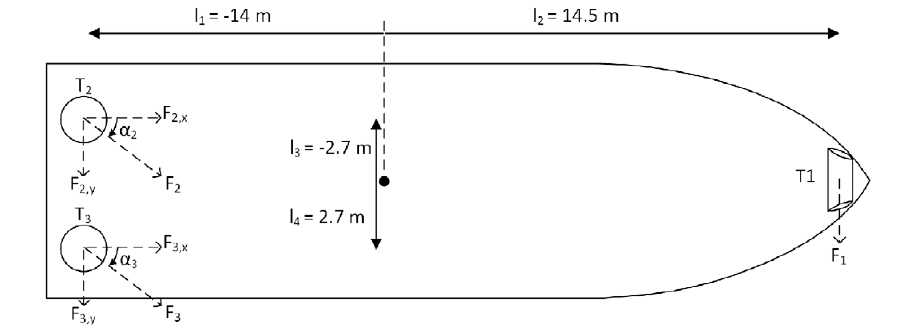
\includegraphics[width=\textwidth]{./ship.png}
        \caption{}
    \end{subfigure} 
    \begin{subfigure}{0.6\textwidth}
        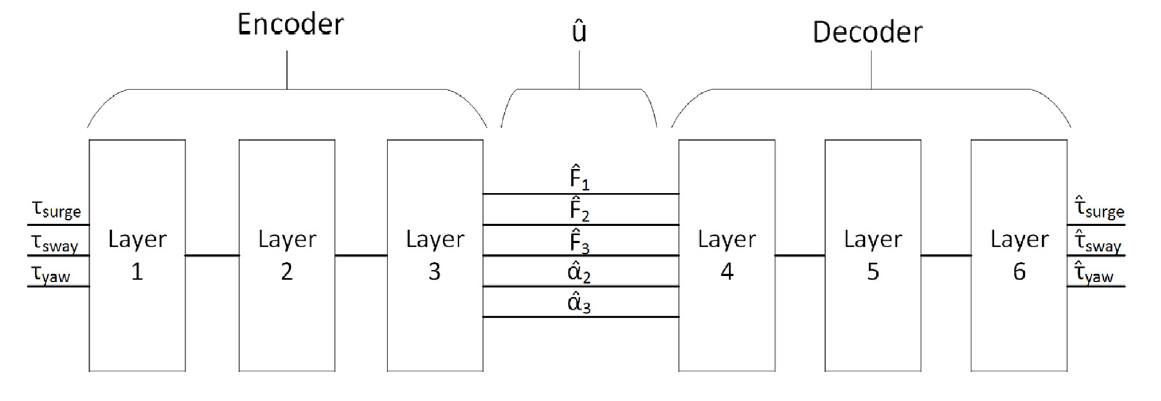
\includegraphics[width=\textwidth]{./autoencoder.png}
        \caption{}
    \end{subfigure}
    \caption{The autoencoder in (b) converts the generalized torques requested from the ship's motion controller to direct commands for the ship's thrusters, $T1$, $T2$, and $T3$ in (b). Since $T1$ is a non-rotatable thruster, only thrusters $T2$ and $T3$ can receive angle commands ($\alpha_2$, and $\alpha_3$).}
    \label{fig:ship}
\end{figure}

While the paper described testing the autoencoder using outputs from a high fidelity ship simulator (which cannot be reproduced for this assignment), the autoencoder was trained using randomly generated data. More specifically, the paper described generating 1 million samples with a randomly initialized random walk for each of the thruster command components, and provided the associated upper and lower bounds. These randomly generated thruster commands were then converted into generalized torque inputs via the following transformation:
\begin{gather*}
    \begin{bmatrix}
        \tau_{surge} \\
        \tau_{sway} \\
        \tau_{yaw}
    \end{bmatrix}
    =
    \begin{bmatrix}
        0 & \cos \left(\alpha_2\right) & \cos \left(\alpha_3\right) \\ 
        1 & \sin \left(\alpha_2\right) & \sin \left(\alpha_3\right) \\
        l_2 & l_1 \sin \left(\alpha_2\right) - l_3 \cos \left(\alpha_2\right) & l_1 \sin \left(\alpha_3\right) - l_4\cos\left(\alpha_3\right)
    \end{bmatrix}
    \dot{}
    \begin{bmatrix}
        F_1 \\
        F_2 \\
        F_3 
    \end{bmatrix}
\end{gather*}
And as part of the autoencoder training, the paper also described a series of different loss functions that were used to drive the output behavior. The separate loss functions were then scaled (according to importance and magnitude via scaling factors $k0$, $k1$, $k2$, $k3$, $k4$, and $k5$, respectively) and combined to form a single loss value to facilitate optimization. The individual loss functions can be described as follows:
\begin{itemize}
    \item $L0$ computed the mean square error (MSE) between the generalized input torques and the torques resulting from directly transforming the encoder's commanded outputs in order to align the inputs with the encoder outputs.
    \item $L1$ computed the MSE between the generalized input torques and the torques output from the decoder in order to align the inputs with the decoder outputs.
    \item $L2$ returned values for individual encoder components that exceeded respective predefined limits in order to minimize the magnitude of the encoder commands.
    \item $L3$ returned values which penalized large rate changes in the encoder commands.
    \item $L4$ computed an estimate of the power output from the encoder commands in an attempt to minimize power consumption.
    \item $L5$ returned values based on the encoder command angle outputs in order to minimize the time that the thrusters are commanded to operate within ``inefficient azimuth sectors''.
\end{itemize}

So in the spirit of using the paper as a starting point, I started implementing the random walk, autoencoder architecture, and loss functions described above in Python. Apart from trying to figure out clever ways to vectorize some of the operations across the massive sample set, implementing the random walk for the input torques described in the paper was pretty straight forward. Along the way, I discovered a workaround for Pytorch's \textit{vmap()} function from a GitHub issue report \cite{github}. While I discovered that the workaround was still limited in its use, I was able to use my custom \textit{vmap()} function to successfully vectorize operations within the sample generation and loss function code without needing to perform millions of loops or broadcast to unfeasable dimensions. Also, while implementing code for shuffling the sample data, I realized that the loss function described by $L3$ in the paper wouldn't apply for this assignment since we don't have any reference for a reasonable time step between samples. In this way, I ended up using somewhat arbitrary step values for my random walk which required minimal course correction when the path for any of the command components strays out of bounds.

For the autoencoder, I initially implemented a class containing LSTM layers. While I was able to get the dimensionality of the LSTMs correct for facilitating the desired number of inputs and outputs of the encoder/decoder, I soon realized that I was over my head. The lecture material prior to this assignment did not cover LSTMs yet, so I was lost when it came to troubleshooting/debugging issues with my autoencoder implementation. So I decided to implement another autoencoder class using all fully connected linear network (FCN) layers because it would be more intuitive for me to troubleshoot and apply regularization techniques to FCNs. While I used the 3 layer encoder/decoder described in the paper as a starting point, I tinkered with the number of layers and neurons in order to help minimize some of the large losses I was seeing (more on this in the next paragraph). I also tinkered with input normalization to the autoencoder, and tinkered with batch normalization and dropout modules within the hidden layers (I made sure to put the batchnorm module after the activation function module when combined with the dropout). 

The loss functions were the hardest part to integrate within my code. While the implementation of the loss functions wasn't too difficult, getting the outputs to cooporate with my FCN model was troublesome. Using the loss function scaling factors that were provided in the paper, I was seeing the gradient of my autoencoder blow up during training. I tinkered with different optimizers and gradient clipping to alleviate this \textemdash\space and I even tinkered with normalizing and scaling the target (truth) data during training despite it being bad practice to do so! Eventually, I discovered that I needed to tinker with the loss function scaling factors for $L0$ and $L1$ since the transform applied to the encoder commands would cause $\tau_{yaw}$ to be disproportionately large compared to the other torques. Once I started tinkering with those scaling factors and minimizing the losses enough, I also began tinkering with a scheduler to apply learning rate decay.

\section{Results}
While I certainly had to cut things short and accept my results as ``good enough'' due to time constraints for the scope of this assignment, the final outputs for my autoencoder can be seen in Figures \ref{fig:tau} through \ref{fig:trval}. Pertinent hyperparameters and design decisions for my autoencoder model contained within my code implementation (control\_allocator.py) are highlighted below:
\begin{outline}
    \1 My encoder implementation contained 5 sequential layers:
        \2 Input linear layer with 3 input features and 60 output features
        \2 1st Hidden linear layer with 60 input features and 90 output features
        \2 2nd Hidden linear layer with 90 input features and 30 output features
        \2 3rd Hidden linear layer with 30 input features and 10 output features
        \2 Output linear layer with 10 input features and 5 output features
        \2 The Input and Hidden layers were all followed by ReLU activation functions before proceeding to the next layer in sequence
        \2 (The Input and Hidden layer activation functions were also all followed by Dropout modules, but the final dropout probability applied across the network was set to 0.0)
    \1 My decoder implementation contained 5 sequential layers that mirrored the encoder:
        \2 Input linear layer with 5 input features and 10 output features
        \2 1st Hidden linear layer with 10 input features and 30 output features
        \2 2nd Hidden linear layer with 30 input features and 90 output features
        \2 3rd Hidden linear layer with 90 input features and 60 output features
        \2 Output linear layer with 60 input features and 3 output features
        \2 The Input and Hidden layers were all followed by ReLU activation functions before proceeding to the next layer in sequence
        \2 (The Input and Hidden layer activation functions were also all followed by Dropout modules, but the final dropout probability applied across the network was set to 0.0)
    \1 I implemented my own custom loss function module with all loss function scaling factors the same as the paper, except for those associated with MSE over the encoder and decoder outputs:
        \2 $k0$ was changed to $10e-9$
        \2 $k1$ was changed to $10e-9$
        \2 (The loss function for rate was also ignored, so the combined loss function became $L = k0L0 + k1L1 + k2L2 + k4L4 + k5L5$)
    \1 I performed a 70/10/20 split of the samples data for Training/Validation/Test:
        \2 I shuffled the training data but left the validation and test data unshuffled
    \1 I used the ADAM optimizer (\textit{optim.Adam()}) with a learning rate of 0.001
    \1 I applied learning rate (\textit{optim.lr\_scheduler.ReduceLROnPlateau()}) decay based on Validation outputs
    \1 I trained for 100 epochs
    \1 I used a batch size of 2000
\end{outline}

\begin{figure}[H]
    \centering
    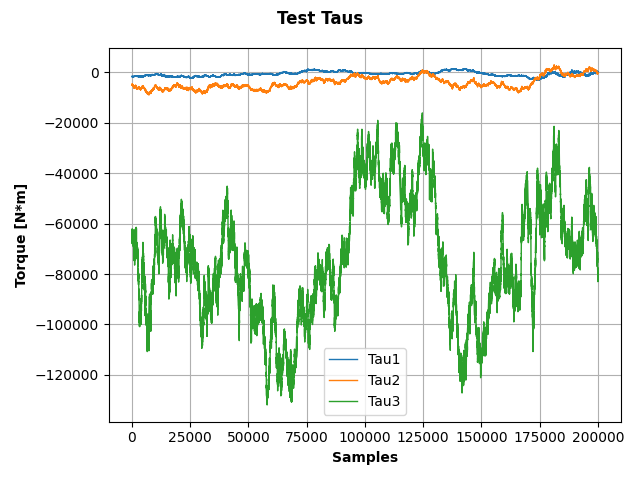
\includegraphics[scale=0.65]{../best_outputs/tau_fig.png}
    \caption{Input Torque Values for the Test Dataset}
    \label{fig:tau}
\end{figure}

\begin{figure}[H]
    \centering
    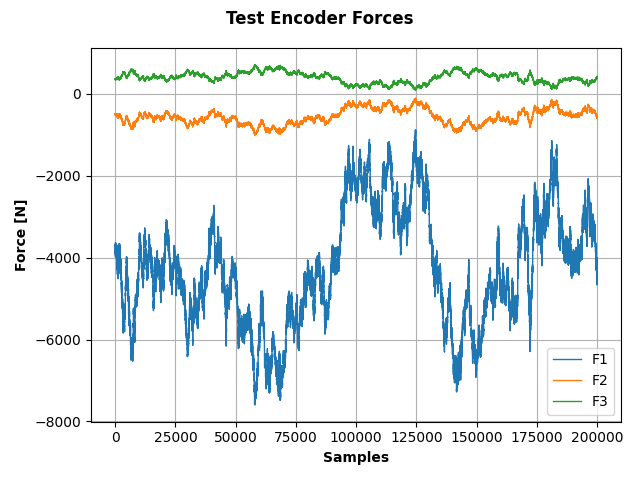
\includegraphics[scale=0.65]{../best_outputs/forces_fig.png}
    \caption{Model Output Forces for the Test Dataset}
    \label{fig:forces}
\end{figure}

\begin{figure}[H]
    \centering
    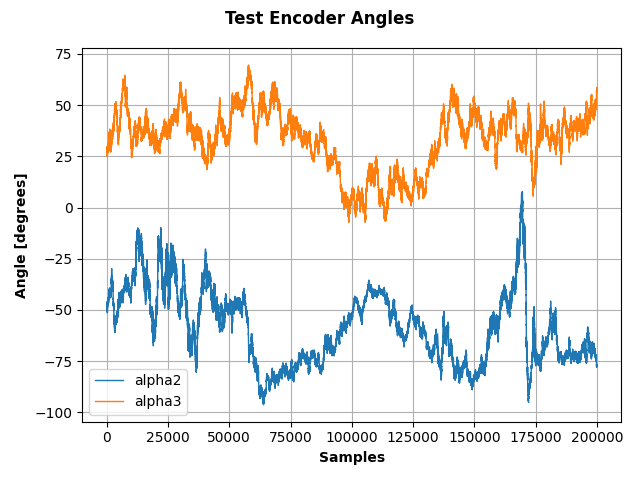
\includegraphics[scale=0.65]{../best_outputs/angles_fig.png}
    \caption{Model Output Angles for the Test Dataset}
    \label{fig:angles}
\end{figure}

\begin{figure}[H]
    \centering
    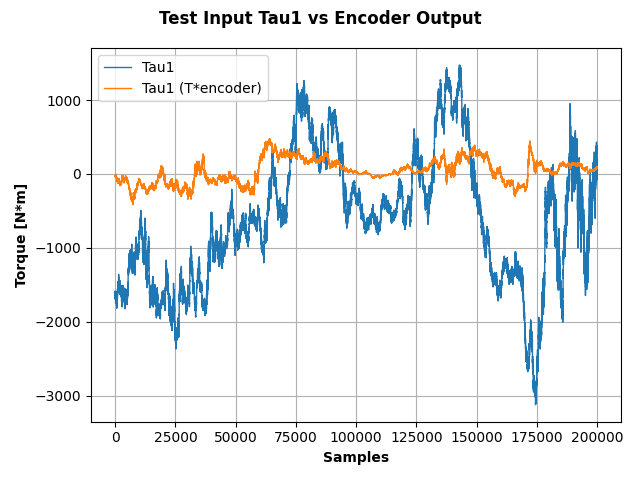
\includegraphics[scale=0.65]{../best_outputs/transform1_fig.png}
    \caption{Test Input $\tau_{surge}$ vs. Transformed Encoder Output}
    \label{fig:transform1}
\end{figure}

\begin{figure}[H]
    \centering
    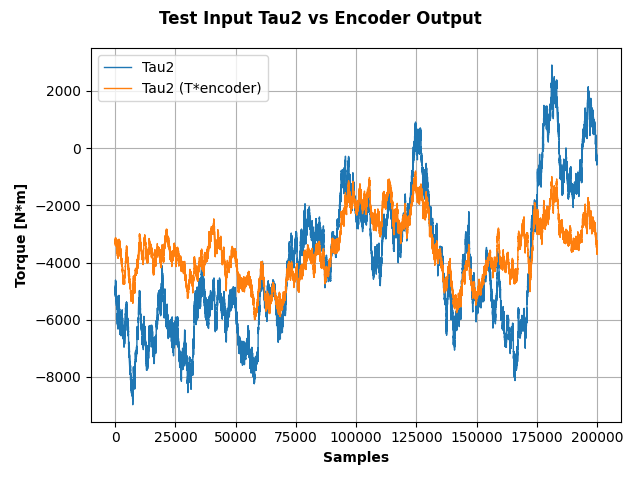
\includegraphics[scale=0.65]{../best_outputs/transform2_fig.png}
    \caption{Test Input $\tau_{sway}$ vs. Transformed Encoder Output}
    \label{fig:transform2}
\end{figure}

\begin{figure}[H]
    \centering
    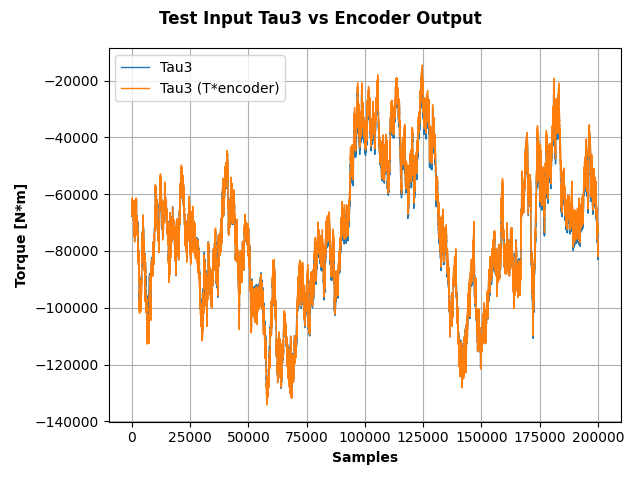
\includegraphics[scale=0.65]{../best_outputs/transform3_fig.png}
    \caption{Test Input $\tau_{yaw}$ vs. Transformed Encoder Output}
    \label{fig:transform3}
\end{figure}

\begin{figure}[H]
    \centering
    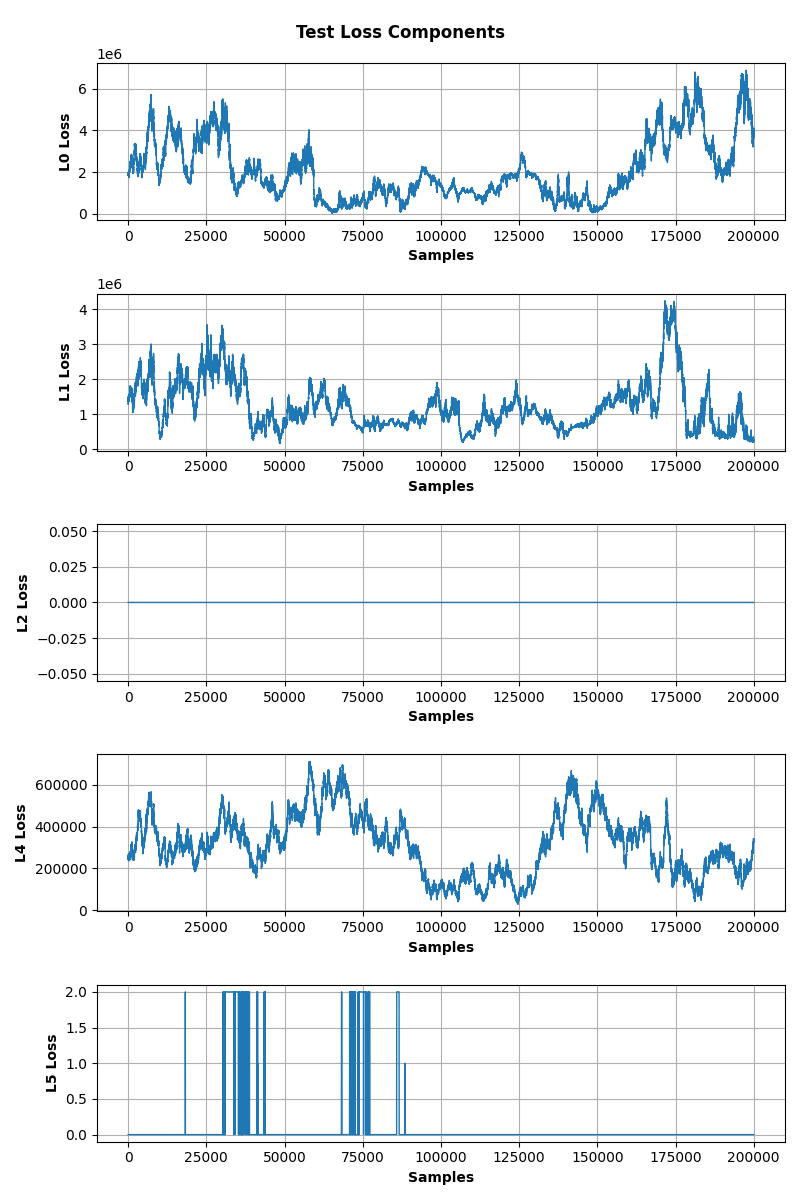
\includegraphics[scale=0.65]{../best_outputs/losses_fig.png}
    \caption{Loss Function Output Components for the Test Dataset}
    \label{fig:losses}
\end{figure}

\begin{figure}[H]
    \centering
    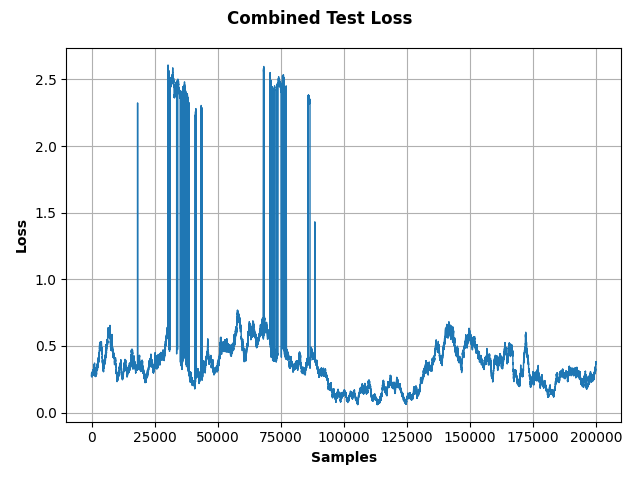
\includegraphics[scale=0.65]{../best_outputs/test_fig.png}
    \caption{Combined Loss Function Output for the Test Dataset}
    \label{fig:test}
\end{figure}

\begin{figure}[H]
    \centering
    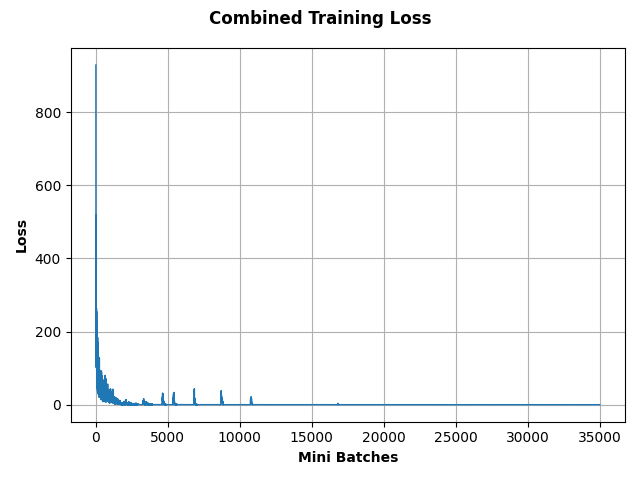
\includegraphics[scale=0.65]{../best_outputs/train_fig.png}
    \caption{Combined Loss Across All Mini Batches for the Training Dataset}
    \label{fig:train}
\end{figure}

\begin{figure}[H]
    \centering
    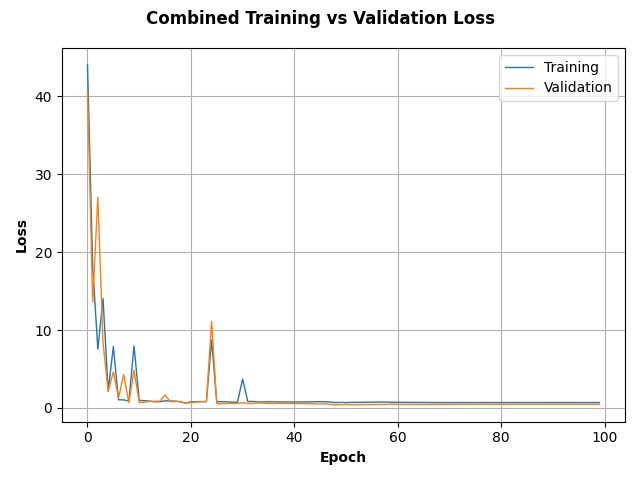
\includegraphics[scale=0.65]{../best_outputs/trval_fig.png}
    \caption{Training and Validation Loss as a Function of Epoch}
    \label{fig:trval}
\end{figure}

\begin{thebibliography}{99}
    \bibitem{paper} Skulstad, R. (2023) (PDF) \textit{constrained control allocation for dynamic ship positioning using Deep Neural Network}, ResearchGate. Available at: \url{https://www.researchgate.net/publication/369978600\_Constrained\_Control\_Allocation\_for\_Dynamic\_Ship\_Positioning\_using\_Deep\_Neural\_Network}. 
    \bibitem{github} Zdevito (2022) \textit{`\_\_getitem\_\_' fails to vmap for one dimensional tensors - ISSUE \#124423 - Pytorch/Pytorch}, GitHub. Available at: \url{https://github.com/pytorch/pytorch/issues/124423}
\end{thebibliography}
\end{document}